\documentclass[12pt, openright,	oneside, a4paper, english, french, spanish, brazil]{abntex2}

% ---
% Pacotes
% ---
\usepackage{lmodern}			                    % Usa a fonte Latin Modern
\usepackage[T1]{fontenc}		                  % Seleção de códigos de fonte.
\usepackage[utf8]{inputenc}		                % Codificação do documento (conversão automática dos acentos)
\usepackage{indentfirst}		                  % Indenta o primeiro parágrafo de cada seção.
\usepackage{color}				                    % Controle das cores
\usepackage{graphicx}			                    % Inclusão de gráficos
\usepackage{microtype} 			                  % para melhorias de justificação
\usepackage[brazilian,hyperpageref]{backref}	% Paginas com as citações na bibl
\usepackage[alf]{abntex2cite}	                % Citações padrão ABNT

% ----------------------------------------------------------
% IMPORTES DE CONFIGURAÇÕES
% ----------------------------------------------------------
% ---
% CONFIGURAÇÕES DE PACOTES
% ---

% ---
% Configurações do pacote backref
% Usado sem a opção hyperpageref de backref
\renewcommand{\backrefpagesname}{Citado na(s) página(s):~}
% Texto padrão antes do número das páginas
\renewcommand{\backref}{}
% Define os textos da citação
\renewcommand*{\backrefalt}[4]{
	\ifcase #1 %
		Nenhuma citação no texto.%
	\or
		Citado na página #2.%
	\else
		Citado #1 vezes nas páginas #2.%
	\fi}%
% ---

% ---
% Configurações de aparência do PDF final

% alterando o aspecto da cor azul
\definecolor{black}{RGB}{0,0,0}

% informações do PDF
\makeatletter
\hypersetup{
     	%pagebackref=true,
		pdftitle={\@title},
		pdfauthor={\@author},
    	pdfsubject={\imprimirpreambulo},
	    pdfcreator={LaTeX with abnTeX2},
		pdfkeywords={abnt}{latex}{abntex}{abntex2}{trabalho acadêmico},
		colorlinks=true,       		% false: boxed links; true: colored links
    	linkcolor=black,          	% color of internal links
    	citecolor=black,        		% color of links to bibliography
    	filecolor=magenta,      		% color of file links
		urlcolor=black,
		bookmarksdepth=4
}
\makeatother
% ---

% ---
% Posiciona figuras e tabelas no topo da página quando adicionadas sozinhas
% em um página em branco. Ver https://github.com/abntex/abntex2/issues/170
\makeatletter
\setlength{\@fptop}{5pt} % Set distance from top of page to first float
\makeatother
% ---

% ---
% Espaçamentos entre linhas e parágrafos
% ---

% O tamanho do parágrafo é dado por:
\setlength{\parindent}{1.3cm}

% Controle do espaçamento entre um parágrafo e outro:
\setlength{\parskip}{0.2cm}  % tente também \onelineskip

% ---
% compila o indice
% ---
\makeindex
% ---

% ----------------------------------
% --- Configurações da capa
% ----------------------------------
\renewcommand{\imprimircapa}{%
    \begin{capa}%
        \center
        \begin{figure*}
            \centering
            
\includegraphics[height=2.5cm]{images/infnet.png}
        \end{figure*}
        \vspace*{\fill}
        {\ABNTEXchapterfont\large\imprimirautor}\\
        \vspace*{\fill}
        \vspace{2.5cm}{\ABNTEXchapterfont\bfseries\LARGE\imprimirtitulo}\\
        \vspace*{\fill}
        \vspace*{\fill}
        \vspace{2.5cm}
        {\large\imprimirlocal}\\
        \par
        {\large\imprimirdata}\\
        \vspace*{1cm}
    \end{capa}
}

% ---
% Informações de dados para CAPA e FOLHA DE ROSTO
% ---

% Título
\titulo{Projeto de Bloco:\\Desenvolvimento Back-End}

% Autores
\autor{Nathan Vieira de Souza}
\local{Ibatiba - ES}
\data{2023}
\orientador{Prof. Elberth Lins Costa de Moraes}
% \coorientador{}
\instituicao{%
  Instituto Infnet
  \par
  Engenharia de Software}

% Tipo de trabalho Monografia de Conclusão de Curso, Tese de Doutorado, Dissertação de Mestrado etc.
\tipotrabalho{Assessment}


% ----------------------------------------------------------
% DOCUMENTO
% ----------------------------------------------------------

% ----
% Início do documento
% ----
\begin{document}

% Seleciona o idioma do documento (conforme pacotes do babel)
\selectlanguage{brazil}

% Retira espaço extra obsoleto entre as frases.
\frenchspacing

% ----------------------------------------------------------
% ELEMENTOS PRÉ-TEXTUAIS
% ----------------------------------------------------------
% \pretextual

% ---
% Capa
% ---
\imprimircapa
% ---

% ---
% Resumo
% ---
\setlength{\absparsep}{18pt} % ajusta o espaçamento dos parágrafos do resumo
\begin{resumo}

  O projeto escolhido é um sistema para facilitar a construção de hábitos com um gestor de tarefas, como ler um livro,
  fazer atividade física ou aprender uma nova lingua, por meio de pequenos objetivos recorrentes ou pontuais ao longo do
  tempo. O foco principal é oferecer uma ferramenta que ajude a formação de hábitos durante a rotina do usuário, de forma
  que ele consiga se manter motivado a alcançar suas metas de longo prazo, ao mesmo tempo, sem se perder nas tarefas
  pontuais que possam aparecer durante esse período. O objetivo final desse projeto é criar uma aplicação que entregue
  para os clientes uma forma de visualizar o seu progresso na criação de um novo hábito, de forma que ele consiga adequar
  a construção desse objetivo durante o seu dia-a-dia, de forma fácil, prática, motivadora e inteligente. Através dessa
  plataforma, a empresa poderá oferecer esse serviço gratuitamente, e avançar com novas funcionalidades, ofertando um
  serviço de assinatura.

 \textbf{Palavras-chave}: Criação de rotinas; criação de hábitos; gestor de tarefas;
\end{resumo}

% ---

% ----------------------------------------------------------
% ELEMENTOS TEXTUAIS
% ----------------------------------------------------------
\textual

% \chapter{Definições}

\section{Tarefa:}

Uma tarefa é uma atividade a ser realizada em um dia, podendo ou não, ser
associada a um intervalo de tempo onde será cumprida. Caso não associada a um
intervalo de tempo, as tarefas podem se acumular para o próximo dia. Exemplo:

\begin{itemize}
  \item{Fazer o trabalho da faculdade}
  \item{Participar da reunião com os fornecedores - 13hrs até as 15hrs}
\end{itemize}


\section{Período:}

Nesse projeto, iremos considerar um período como o espaço de tempo em dias que
transcorre entre duas tarefas semelhantes.

\section{Rotina:}

Uma rotina, também pode ser chamado de tarefa periódica, é um conjunto de tarefas
semelhantes que se replicam após um \textbf{período} pré-definido. Exemplo:

\begin{itemize}
  \item{Ler o jornal diáriamente}
  \begin{itemize}
    \item{Dia 1: Ler o jornal}
    \item{Dia 2: Ler o jornal}
    \item{Dia n: Ler o jornal}
  \end{itemize}
\end{itemize}

\section{Repetição:}

Nesse projeto, iremos considerar uma repetição como a unidade de uma tarefa que
compõe uma \textbf{rotina}.

\newpage

\section{Objetivo:}

Um objetivo é uma rotina que possuí uma meta quantitativa. Nesse caso, ao concluir
cada \textbf{repetição}, deve-se informar o avanço realizado. Exemplo:

\begin{itemize}
  \item{Ler o livro Código Limpo - 425 Páginas}
  \begin{itemize}
    \item{Dia 1: Ler o livro Código Limpo - Foi lido +10 páginas}
    \item{Dia 2: Ler o livro Código Limpo - Foi lido +30 páginas}
    \item{Dia n: Ler o livro Código Limpo - Foi lido +100 páginas}
  \end{itemize}
\end{itemize}

\section{Ciclo:}

Nesse projeto, um ciclo são 22 dias consecutivos de repetições sendo realizadas.
A tolerância para repetições não realizadas, deve depender da quantidade de ciclos
já atingidos.

\section{Hábito:}

Um hábito é composto por vários objetivos ou rotinas. Esses hábitos devem ser
mensurados em dias e categorizados em ciclos. Exemplo:

\begin{itemize}
  \item{Hábito de ler:}
  \begin{itemize}
    \item{Ler o jornal diáriamente \textbf{(rotina)}}
    \begin{itemize}
      \item{Dia 1: Ler o jornal}
      \item{Dia 2: Ler o jornal}
      \item{Dia n: Ler o jornal}
    \end{itemize}
    \item{Ler o livro Código Limpo - 425 Páginas \textbf{(objetivo)}}
    \begin{itemize}
      \item{Dia 1: Ler o livro Código Limpo - Foi lido +10 páginas}
      \item{Dia 2: Ler o livro Código Limpo - Foi lido +30 páginas}
      \item{Dia n: Ler o livro Código Limpo - Foi lido +100 páginas}
    \end{itemize}

  \end{itemize}
\end{itemize}

\section{Programação:}

Nesse projeto, uma programação se refere a qualquer tipo de evento que esteja
programado. Ou seja, qualquer tarefa, rotina, repetição, objetivo ou hábito.



\chapter{Principais funcionalidades}

\section{Requisitos funcionais:}
\begin{description}

  \item[Gestão de tarefas:] O cliente deve conseguir administrar uma tarefa
    em sua conta. Podendo atribuir, ou não, um intervalo de tempo a essa tarefa e
    também definir se a tarefa irá se acumular para o próximo dia, caso não
    realizada.

  \item[Gestão de rotinas:] O cliente deve ser capaz de administrar as rotinas
    de sua conta. Definindo o período de cada repetição, e a tarefa que irá ser repetida.
    Para que isso seja possível, deve-se acrescentar ao sistema de gestão de tarefas,
    a estrutura para uma tarefa periódica.

  \item[Gestão de objetivos:] O cliente deve ser capaz de administrar os objetivos
    de sua conta. Definindo o período de cada repetição, a tarefa que irá ser repetida
    e as metas que irá ser alcançada. Para que isso seja possível, deve-se acrescentar
    ao sistema de gestão de tarefas, o registro quantitativo do progresso.

  \item[Gestão de hábitos:] O cliente deve ser capaz de administrar os hábitos
    em sua conta, definir as rotinas ou objetivos que serão repetidos. Também será
    necessário adicionar ao sistema de progresso, a possibilidade de reiniciar o
    avanço caso a tolerância de repetições do ciclo seja excedida.

  \item[Sistema de aviso:] O cliente deve ser capaz de configurar quais
  tarefas, rotinas ou hábitos. Que vão acionar uma notificação/alerta quando
  estiver próximo ao horário planejado para a o evento.

\end{description}

\newpage

\section{Requisitos não funcionais:}

\begin{description}
  \subsection*{Segurança}

  \item[Autenticação:] O cliente deve ser capaz de se cadastrar e autenticar no
    sistema, fornecendo informações básicas, como nome, e-mail e senha.

  \subsection*{Usabilidade}

  \item[Interface amigável:] O sistema deve possuir uma interface de usuário web e
  mobile, que facilite a utilização e navegação.

  \item[Sistema de progresso:] O sistema deve ser capaz de mostrar o progresso
    dos objetivos de forma quantitativa, enquanto as rotinas e os hábitos devem ter
    o progresso exibido utilizando ciclo atual e o avanço no ciclo.

  \subsection*{Disponibilidade}

  \item[Suporte ao cliente:] O sistema deve oferecer suporte ao cliente, com
  opções de contato para dúvidas, problemas ou qualquer assistência necessária.

  \subsection*{Interoperabilidade}

  \item[Integração:] O cliente deve conseguir sincronizar suas programações com
  serviços externos, como Google Calendar e/ou com outros serviços do gênero.

\end{description}


\chapter{Organizações das entregas}

\begin{enumerate}
  \item Primeira entrega:

  \begin{itemize}
    \item{Autenticação}
    \item{Gestão de tarefas}
    \item{Gestão de rotinas}
  \end{itemize}

  \item Segunda entrega:

  \begin{itemize}
    \item{Interface Amigável}
    \item{Gestão de objetivos}
    \item{Sistema de progresso}
    \item{Gestão de hábitos}
  \end{itemize}

  \item Terceira entrega:

  \begin{itemize}
    \item{Sistema de aviso}
    \item{Suporte ao cliente}
    \item{Integração com outros serviços externos}
  \end{itemize}
\end{enumerate}


\chapter{Diagrama de caso de uso}

\begin{figure}[h]
  \centering
  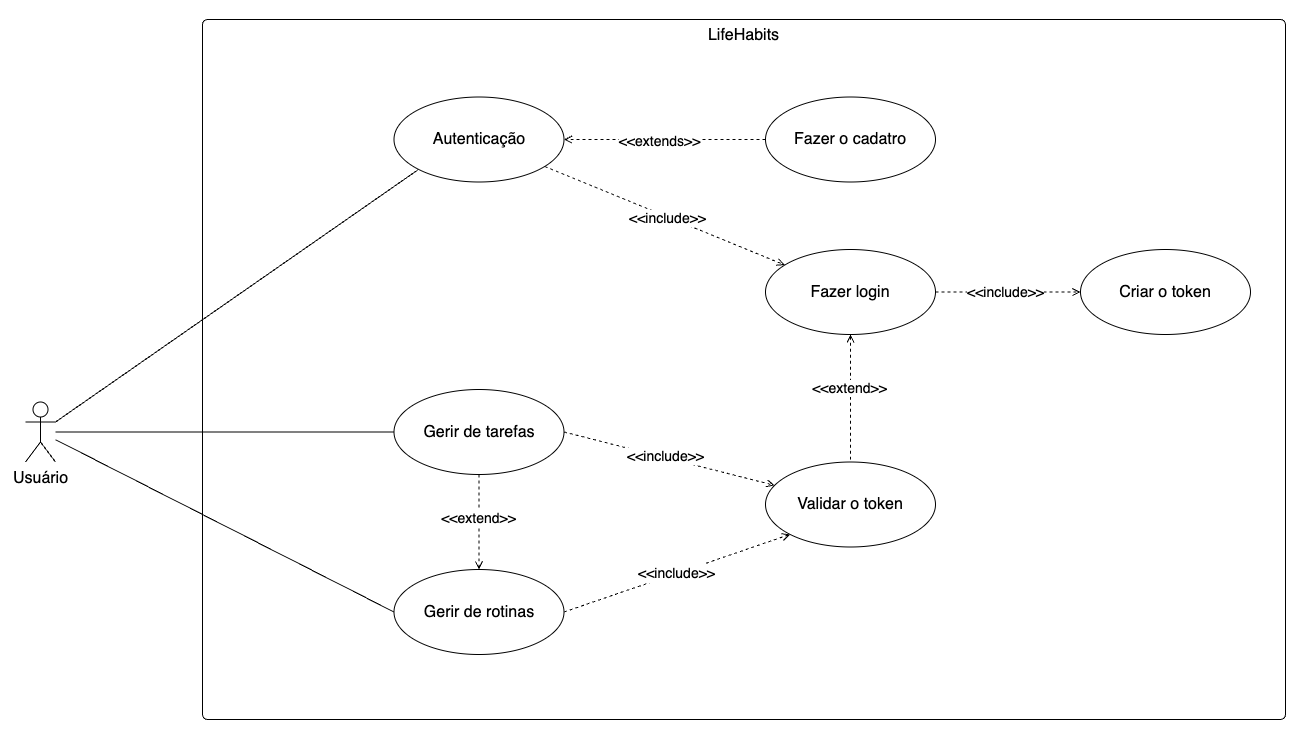
\includegraphics[scale=0.34]{images/diagrams/use-case.png}
\end{figure}



\chapter{Entidades}

% User
\section{Usuário (User)}

\textbf{Descrição:} O usuário é o ator do sistema, ele será o sujeito que poderá gerenciadas a grande
maioria das entidades.

\textbf{Campos:} id, email, name, created\_at, updated\_at

\textbf{Relacionamento:} Um usuário tem uma agenda (e todos os seus eventos), uma credencial e vários rotinas, hábitos ou objetivos.

% Schedule
\section{Agenda (Schedule)}

\textbf{Descrição:} A agenda é responsável por registrar o cronograma e organizar os eventos em um calendário.

\textbf{Campos:} id, events

\textbf{Relacionamento:} Um usuário possuí uma agenda, e uma agenda possuí vários eventos

% ScheduleEvent
\section{\textit{Evento Agendado (ScheduleEvent)}}

\textbf{Descrição:} Evento Agendado é uma classe abstrata que representa qualquer alocação de tempo em uma agenda.

\textbf{Campos:} id, schedule\_id, title, description, status, start\_at, end\_at

\textbf{Relacionamento:} Um evento agendado pertence a uma agenda, podendo ser uma tarefa ou uma interação.

% Task
\section{Tarefa (Task)}

\textbf{Descrição:} Uma Tarefa é um tipo de evento agendado que irá acontecer apenas uma vez.

\textbf{Campos:} expire\_at

\textbf{Relacionamento:} Uma tarefa é um tipo de evento agendado, portanto pertence a uma agenda.

% Interaction
\section{Interação (Interaction)}

\textbf{Descrição:} Uma Interação é um tipo de evento agendado que registra as informações referentes a uma repetição de um ciclo.

\textbf{Campos:} cyclo\_id

\textbf{Relacionamento:} Uma tarefa é um tipo de evento agendado, portanto pertence a uma agenda. Ao mesmo tempo, uma interação pertence a um ciclo.

% Cyclo
\section{Ciclo (Cyclo)}

\textbf{Descrição:} Ciclo é um conjunto de repetição, ou seja, um conjunto de eventos agendados semelhantes. Os ciclos possuem tamanho e progresso mensurados em dias.

\textbf{Campos:} id, routine\_id, interactions, size, progress, period

\textbf{Relacionamento:} Um ciclo possuí várias interações, e pertence a uma rotina.

% Routine
\section{Rotina (Routine)}

\textbf{Descrição:} Uma rotina é a entidade que possuí ciclos, e eles são a métrica do progresso dessa entidade. Em uma rotina, toda repetição é importante ser realizada.

\textbf{Campos:} id, title, description, cyclos, status, progress, end\_at

\textbf{Relacionamento:} Uma rotina pode ter vários ciclos e pertence a um usuário.

% Objective
\section{Objetivo (Objetive)}

\textbf{Descrição:} Um objetivo é um tipo de rotina que possuí uma meta muito bem clara.

\textbf{Campos:} id, title, description, cyclos, status, progress, end\_at, progress, magnitude

\textbf{Relacionamento:} Um objetivo pode ter vários ciclos e pertence a um usuário.

% Habit
\section{Hábito (Habit)}

\textbf{Descrição:} Um hábito é um tipo de rotina onde a frequência de realização de cada repetição é muito importante.

\textbf{Campos:} id, title, description, cyclos, status, progress, end\_at

\textbf{Relacionamento:} Um objetivo pode ter vários ciclos e pertence a um usuário.


\chapter{Diagrama de classes}

\begin{figure}[h]
  \centering
  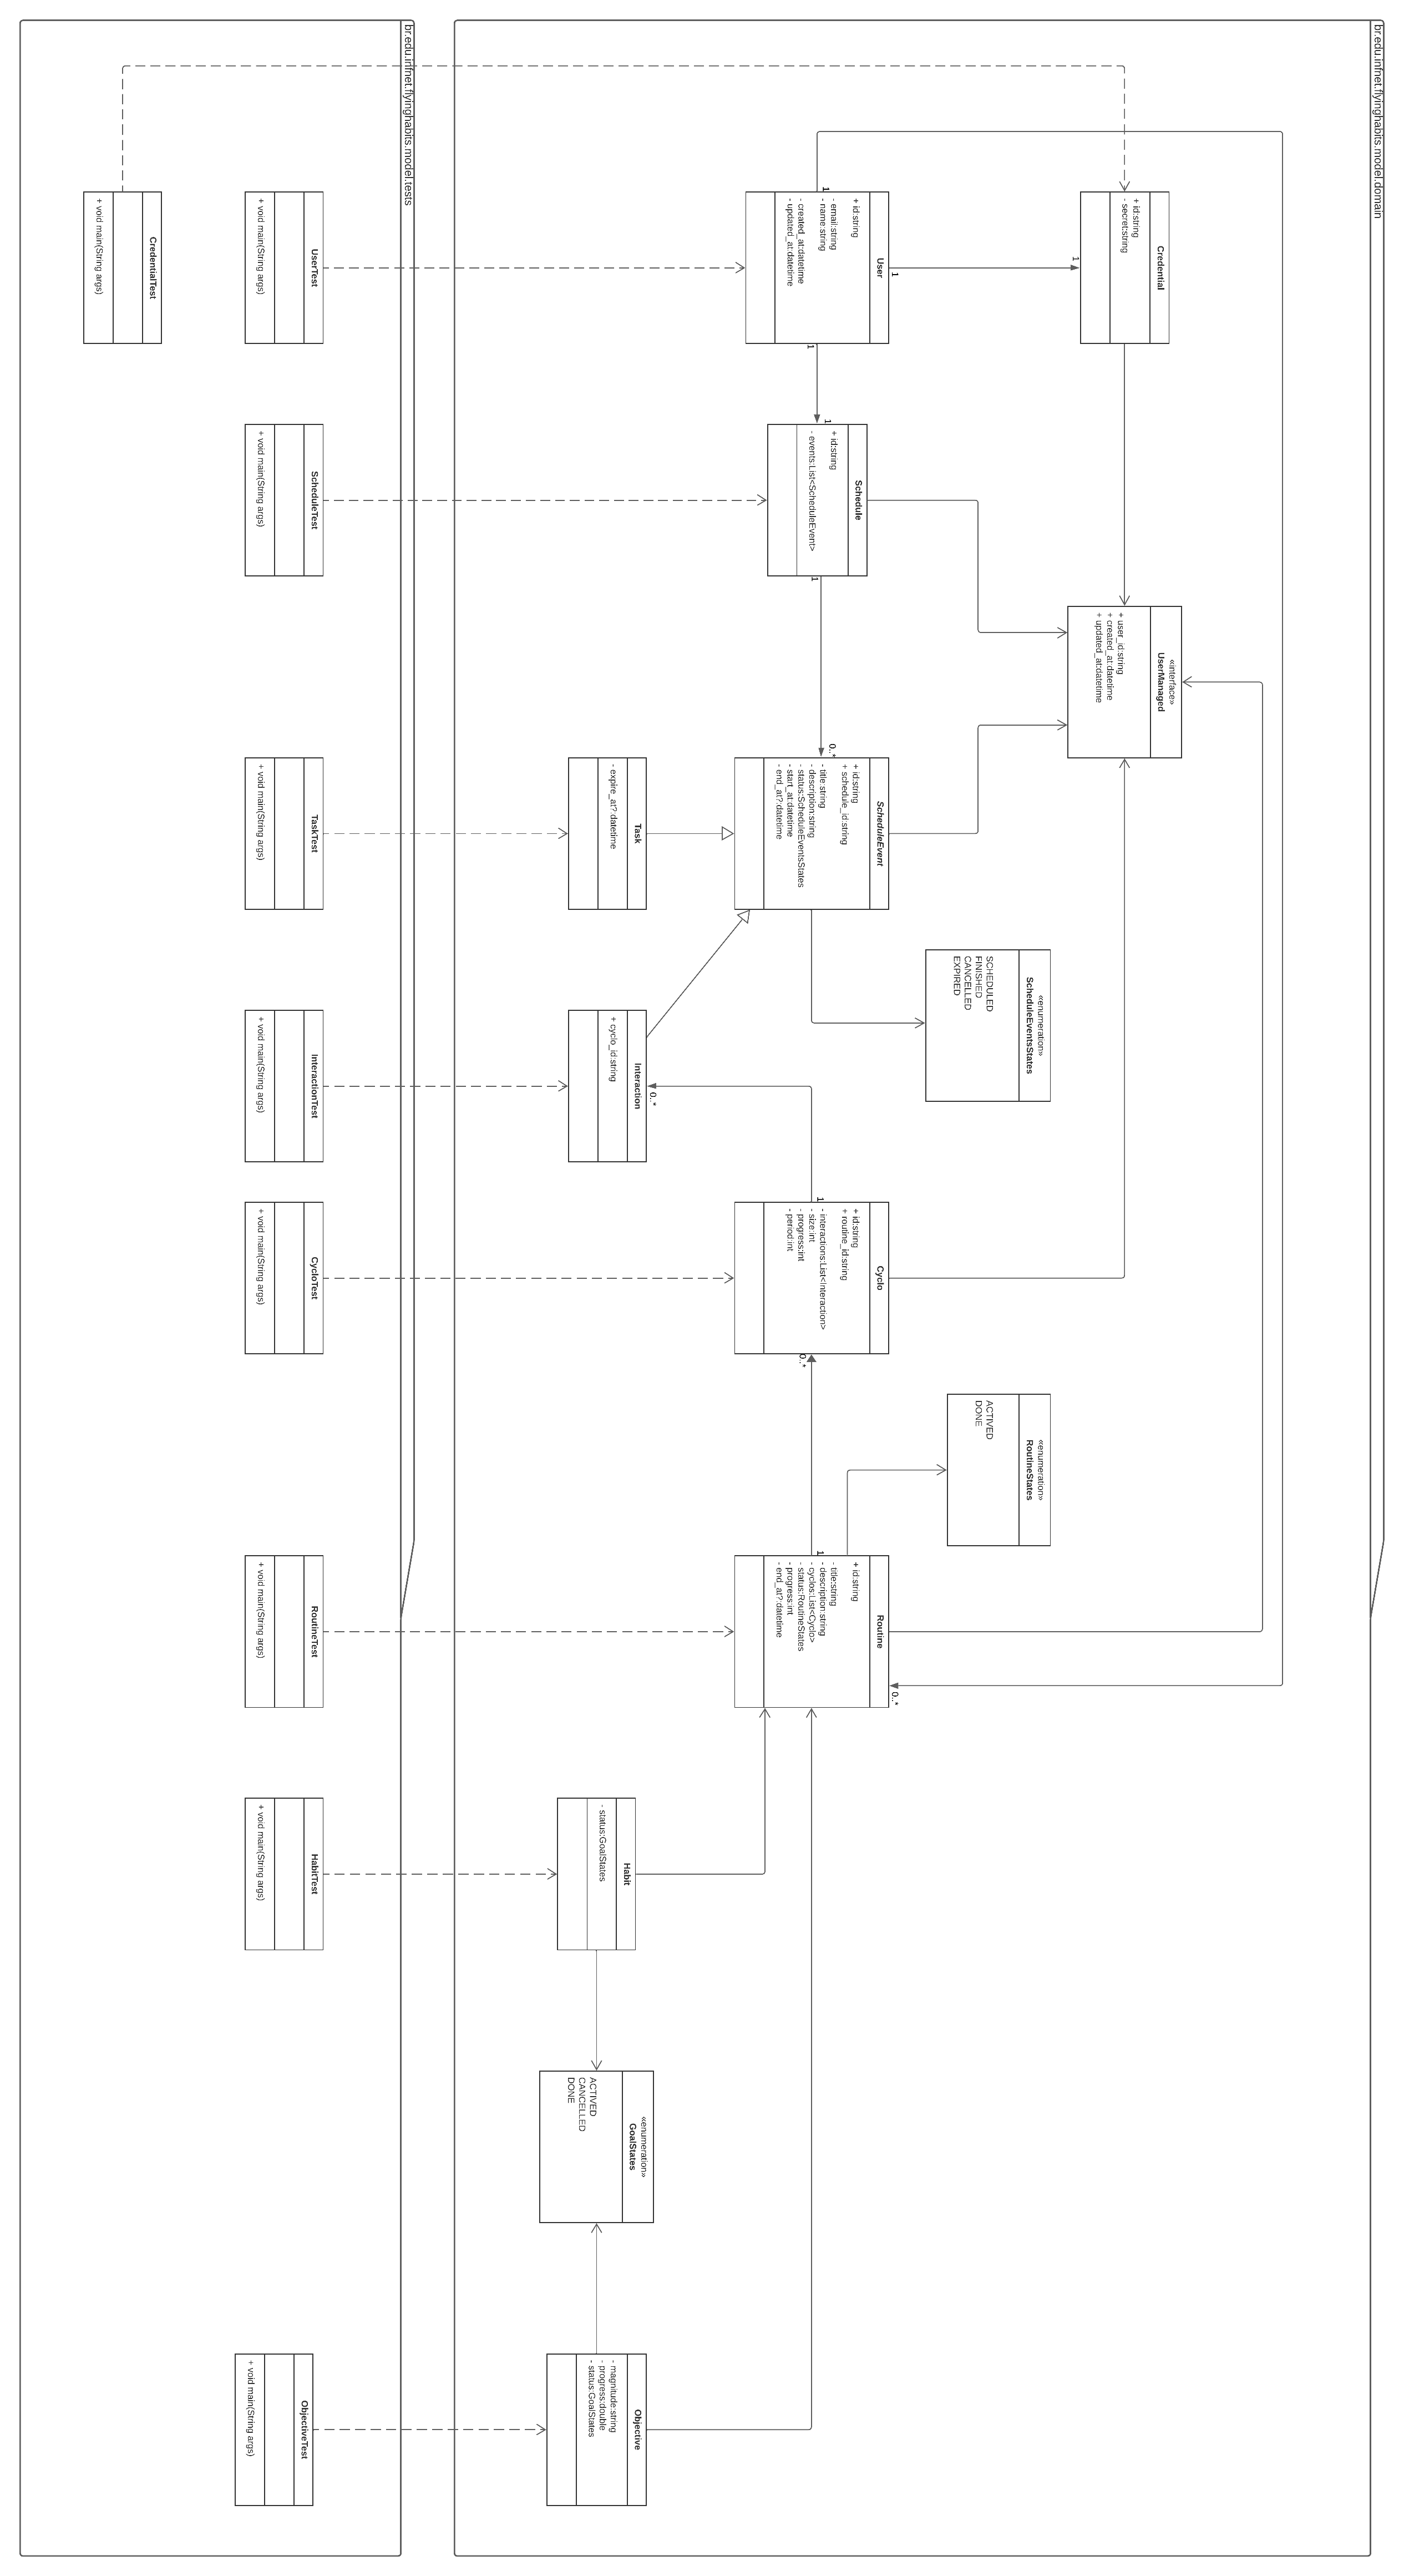
\includegraphics[scale=0.5]{images/diagrams/classes.png}

  \url{https://lucid.app/documents/view/0cdecbc9-72ed-45f9-8ffd-27824700e669}
\end{figure}


\end{document}
